\documentclass{standalone}
\usepackage[utf8]{inputenc}
\usepackage{tikz}
\usepackage{pgfplots}
\usepackage{amsmath}

\begin{document}

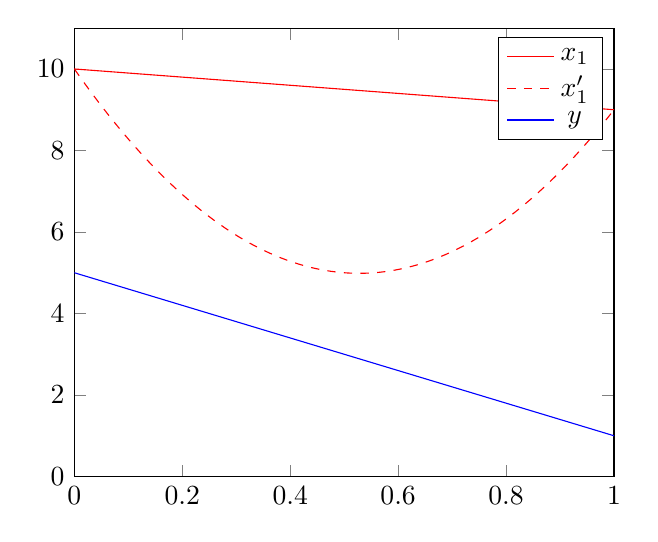
\begin{tikzpicture}
    \begin{axis}[
    xmin=0,xmax=1,
    ymin=0,ymax=11,
    ]
        \addplot[color=red]{-x+10};
        \addlegendentry{$x_1$}
        \addplot[color=red, dashed, domain=0:1, samples=100,]{18*x^2-19*x+10};
        \addlegendentry{$x'_1$}
        \addplot[color=blue]{-4*x+5};
        \addlegendentry{$y$}
    \end{axis}
\end{tikzpicture}

\end{document}
